\input{../../../../.preambles/02-lab_work}
\input{../../../../.preambles/30-physics}
\newgeometry{top=1.5cm, bottom=1.5cm, left=1cm, right=1cm}
\newcommand{\el}[3]{\nucleus{#2}{#3}{#1}}
\begin{document}
    \begin{table}[h!]
        \center
        \begin{tabular}{|C{.5}|C{.2}|C{.25}|}
            \hline
            \multicolumn{1}{|c|}{\multirow{4}{*}{Лабораторная работа № 4}} &
            Студент, группа & {{ student }}, Ф-369 \\ \cline{2-3}
            & Дата выполнения & 06.03.2013 \\ \cline{2-3}
            & Подпись &  \\ \cline{2-3}
            Изучение явления радиоактивности & Дата отчёта & \\ \cline{2-3}
            & Оценка &  \\ \cline{2-3}
            & Подпись &  \\ \hline
        \end{tabular}
    \end{table}

    \emph{Цель работы:} Изучение явления радиоактивности с помощью компьютерного
    моделирования процессов \( \alpha \)- и \( \beta \)-распадов радиоактивных ядер.
    
    \vspace*{2em}
    
    \textbf{Семейство \( A = 4n \):} \( \alpha \)-распад
    \( \el{U}{236}{92} \to \el{Th}{232}{90} \).
    
    \vspace*{1em}
    
    Период полураспада \( \el{U}{236}{92} \):
    \( T_{1/2} = 2,4 \cdot 10^9 \)~лет,
    период полураспада \( \el{Th}{232}{90} \):
    \( T_{1/2} = 1,4 \cdot 10^{10} \)~лет.
    
    \begin{figure}[h!]
        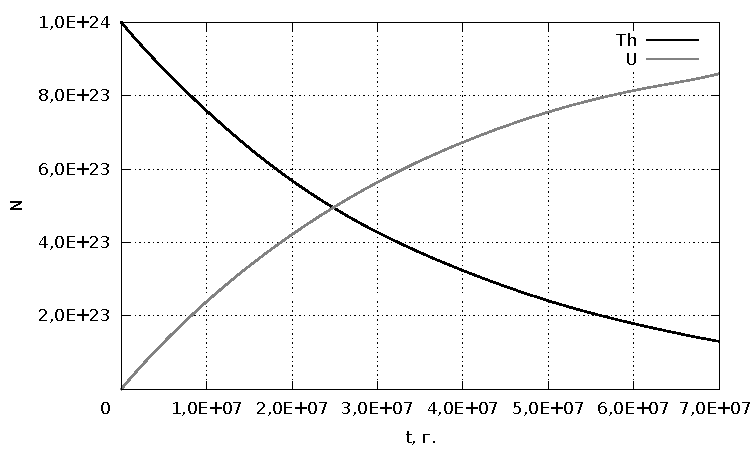
\includegraphics[width=.47\textwidth]{4n_forward} \hfill
        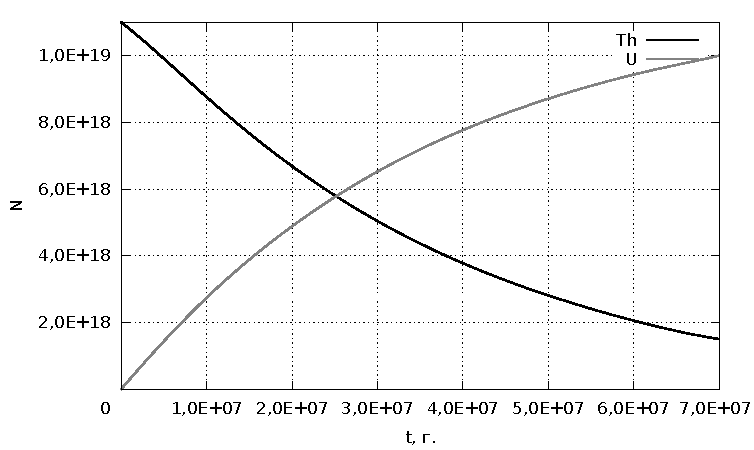
\includegraphics[width=.47\textwidth]{4n_backward}
        \parbox{.47\textwidth}{\caption{Прямая задача, количество начального
        элемента: \( N_\emph{п} = 1 \cdot 10^{24} \)~ядер}} \hfill
        \parbox{.47\textwidth}{\caption{Обратная задача, количество конечного
        элемента: \( N_\emph{ок} = 1 \cdot 10^{19} \)~ядер }}
    \end{figure}
    
    Полученное значение количества конечного элемента в прямой задаче:
    \( N_\emph{пк} = 8,\!6 \cdot 10^{23} \)~ядер.
    
    Полученное значение количества начального элемента в обратной задаче:
    \( N_\emph{о} = 1,\!15 \cdot 10^{19} \)~ядер.
    
    \vspace*{2em}
    
    \textbf{Семейство \( A = 4n + 1\):} \( \beta^- \)-распад
    \( \el{Ra}{225}{88} \to \el{Ac}{225}{89} \).
    
    \vspace*{1em}
    
    Период полураспада \( \el{Ra}{225}{88} \): \( T_{1/2} = 14,\!8 \)~дней,
    период полураспада \( \el{Ac}{225}{89} \): \( T_{1/2} = 10,\!0 \)~дней.
    
    \begin{figure}[h!]
        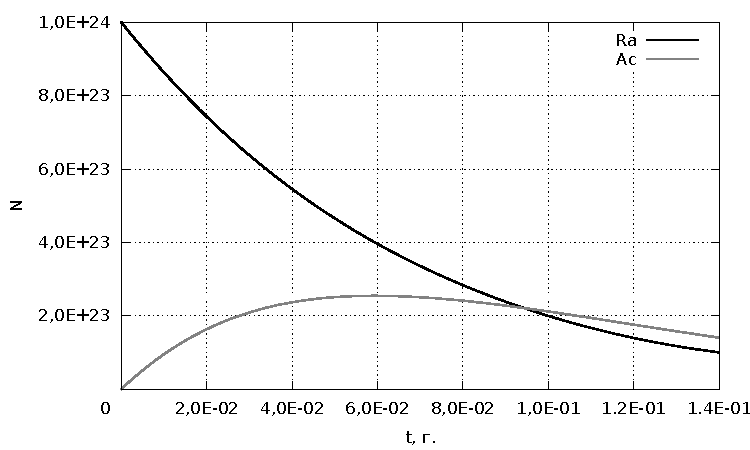
\includegraphics[width=.47\textwidth]{4n+1_forward} \hfill
        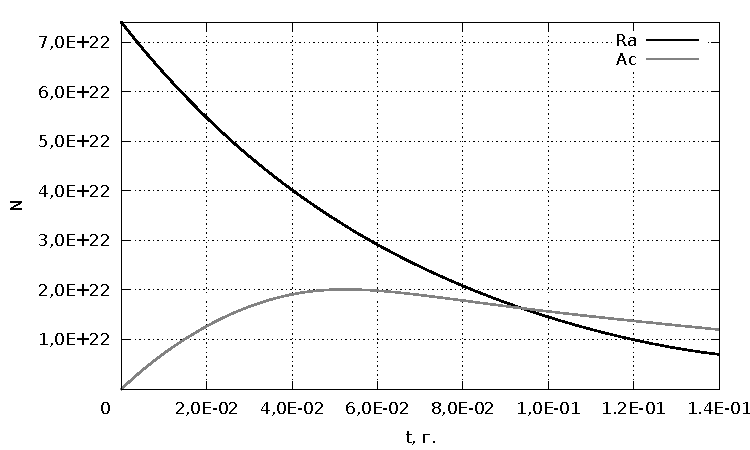
\includegraphics[width=.47\textwidth]{4n+1_backward}
        \parbox{.47\textwidth}{\caption{Прямая задача, количество начального
        элемента: \( N_\emph{п} = 1 \cdot 10^{24} \)~ядер}} \hfill
        \parbox{.47\textwidth}{\caption{Обратная задача, количество конечного
        элемента: \( N_\emph{ок} = 1 \cdot 10^{22} \)~ядер }}
    \end{figure}
    
    Полученное значение количества конечного элемента в прямой задаче:
    \( N_\emph{пк} = 1,\!4 \cdot 10^{23} \)~ядер.
    
    Полученное значение количества начального элемента в обратной задаче:
    \( N_\emph{о} = 7,\!4 \cdot 10^{22} \)~ядер.
    
    \pagebreak
    
    \textbf{Семейство \( A = 4n + 2\):} \( \alpha \)- и \( \beta^- \) распады
    \( \el{Po}{218}{84} \to \el{Pb}{214}{82} \to \el{Bi}{214}{83} \).
    
    \vspace*{1em}
    
    Периоды полураспада: \( \el{Po}{218}{84} \) -- \( T_{1/2} = 3 \)~мин;
    \( \el{Pb}{214}{82} \) -- \( T_{1/2} = 27 \)~мин; \( el{Bi}{214}{83} \) --
    \( T_{1/2} = 20 \)~мин.
    
    \begin{figure}[h!]
        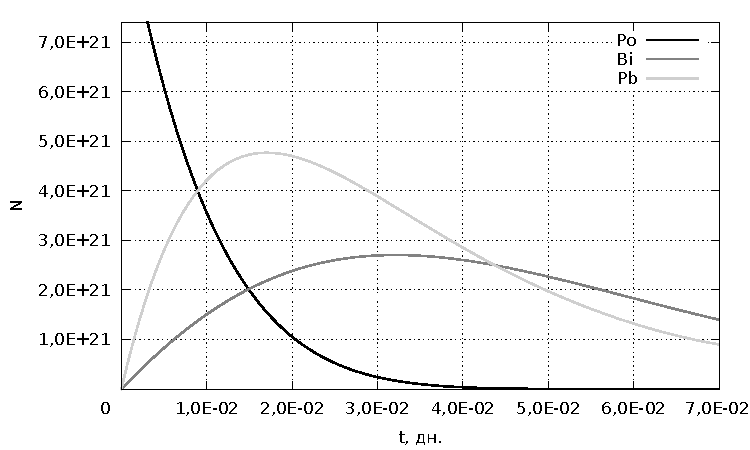
\includegraphics[width=.47\textwidth]{4n+2_forward} \hfill
        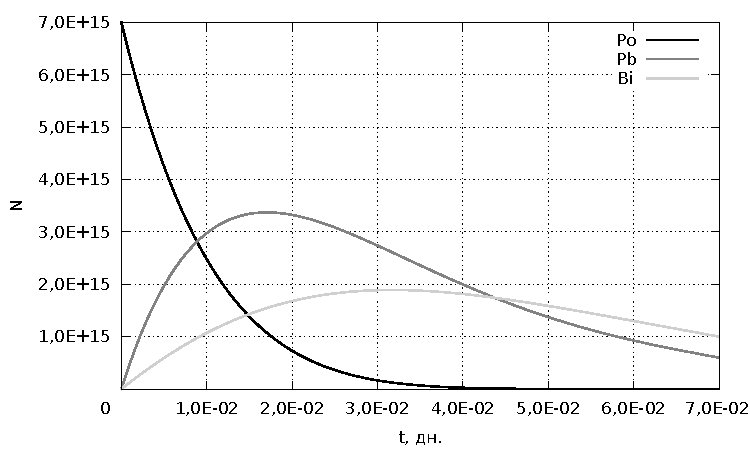
\includegraphics[width=.47\textwidth]{4n+2_backward}
        \parbox{.47\textwidth}{\caption{Прямая задача, количество начального
        элемента: \( N_\emph{п} = 1 \cdot 10^{22} \)~ядер}} \hfill
        \parbox{.47\textwidth}{\caption{Обратная задача, количество конечного
        элемента: \( N_\emph{ок} = 1 \cdot 10^{15} \)~ядер }}
    \end{figure}
    
    Полученное значение количества конечного элемента в прямой задаче:
    \( N_\emph{пк} = 1,\!4 \cdot 10^{21} \)~ядер.
    
    Полученное значение количества начального элемента в обратной задаче:
    \( N_\emph{о} = 7,\!0 \cdot 10^{15} \)~ядер.
    
    \vspace*{2em}
    
    \emph{Вывод:} был проведен опыт по компьютерному моделированию процессов
    \( \alpha \)- и \( \beta \)-распадов радиоактивных ядер, по результатам
    которого были найдены количества начального и конечного элементов,
    совпадающих с теоретическими расчетами.
\end{document}